\chapter[Gestión, planificación y desarrollo del software]{Gestión, planificación y desarrollo del proyecto de software}

En los capítulos anteriores  hemos presentado las bases del testing, de la computación cuántica, de mutation testing y de los principales problemas que aparecen a la hora de adaptar este proceso al mundo cuántico. 
%
En este capítulo presentamos el sistema
\textit{software} desarrollado donde se implementan todas estas ideas. En particular,
hablaremos de gestión, planificación y desarrollo de funcionalidades. La estructura y muchos de los conceptos tratados en este capítulo se sustentan en los conocimientos adquiridos en  distintas asignaturas de la carrera, especialmente en \textit{Ingeniería del Software}. 

\section{Gestión del proyecto}

En primer lugar, vamos a presentar todo el proceso de gestión del proyecto, desde la organización como equipo, hasta herramientas y \textit{software} utilizado para  desarrollar el código y la memoria.

\subsection{Gestión de equipo}

La gestión del equipo es sencilla. Los dos miembros del grupo contamos con el mismo poder para la toma de decisiones y, por tanto, dichas decisiones han de tomarse de manera consensuada. Si bien es cierto que, según la actividad, alguno de los miembros puede estar más involucrado en ella y es razonable que sus argumentos tenga un mayor peso.

Además, en caso de decisiones clave siempre teníamos una segunda opinión: la correspondiente a nuestros tutores.  Por tanto, podemos decir que ellos han formado parte también de la toma de decisiones. Hemos tratado de involucrarnos por igual en todas las fases y tareas del TFG con, tal vez, algunas excepciones. Veremos a continuación de forma detallada la contribución de cada uno de los miembros al proyecto.

\subsection{Contribución al proyecto de Luis Aguirre}
% Al menos dos páginas

La idea de realizar este proyecto comienza a finales de junio de 2019. Nos pusimos en contacto con los directores de este trabajo y se realiza una primera reunión. Hay que mencionar que las dos disciplinas principales sobre las que se ha construido este trabajo, mutation testing y computación cuántica, son áreas sobre las que no habíamos visto ni siquiera una pequeña introducción en alguna de las asignaturas de la carrera de Informática o Matemáticas cursadas hasta la fecha.

Es por ello que a raíz de esta reunión inicial surge una primera tarea a realizar: investigar y adquirir conocimiento sobre mutation testing y computación cuántica. Para ello utilicé como literatura, principalmente, \textit{Introducción a la computación cuántica para no-físicos} [\cite{rieffel2000introduction}]. De este texto obtuve las primeras nociones importantes sobre computación cuántica que se han ido mencionando a lo largo del texto: qubit, superposición de estados, entrelazamiento, paralelismo y un largo etcétera. Además, también se realizó una lectura exhaustiva de un recurso online [\cite{quantumcountry}] desarrollado por uno de los promotores de la computación cuántica más relevantes en la actualidad, Michael A.Nielsen, con la colaboración de Andy Matuschak. Este recurso me pareció adecuado pues la interfaz y el método de lectura están construidas sobre potentes ideas del campo de la ciencia cognitiva y su principal objetivo es hacer que el lector recuerde los nuevos conceptos aprendidos, que en el caso de la computación cuántica suelen tratarse de conceptos y notación que no es familiar.

A su vez, para aprender las primeras ideas del mutation testing se realizó una lectura del artículo \textit{Mutation Testing} [\cite{hierons2010mutation}], si bien más adelante, durante el curso 2019/2020, decidí cursar la asignatura \textit{Testing de Software} con la idea de ampliar mi conocimiento sobre testing y de esta forma poder aplicarlo a este proyecto.

Una vez que se tenían los conceptos principales sobre computación cuántica y mutation testing, se realiza una nueva reunión donde se decide en qué lenguaje cuántico se especializará cada alumno. En mi caso decidí estudiar el lenguaje cuántico de Microsoft \qsh. Esta tarea implicó aprender a instalar el entorno de desarrollo y las distintas alternativas de las que se disponía, familiarizarse con la sintaxis del lenguaje, así como con el sistema de tipado, o examinar ejemplos de código desarrollado por Microsoft. Esta última tarea fue especialmente importante pues me permitió reconocer qué operadores eran más utilizados, siempre con la idea en mente de poder definir un operador de mutación a partir de ellos.

Todo este trabajo es previo a empezar a desarrollar el sistema  y ha sido, posiblemente, la etapa que más tiempo ha consumido. Esto se debe al hecho de haber realizado un trabajo sobre un campo que era prácticamente desconocido para mi, y por ello decidí que era imprescindible dedicar una importante porción del trabajo a la formación y  estudio de este área.

Tras haber realizado el estudio previo, tarea que se alarga hasta principio de 2020, se comienza con el desarrollo del sistema. Este proceso se extenderá a lo largo de tres meses, aproximadamente. La realidad es que ambos componentes del grupo nos hemos involucrado de manera similar en el diseño y creación del programa.

Acostumbrados ya a una dinámica previa de trabajo conjunto, se fueron designando pequeñas tareas que debían ser llevadas a cabo. Este ha sido el proceso que se ha seguido durante todo el desarrollo del sistema y, por tanto, ninguna de las componentes principales del programa ha sido desarrollada única y exclusivamente por alguno de los miembros del grupo. Sin embargo, la responsabilidad de desarrollar alguna de estas pequeñas tareas mencionadas previamente ha podido recaer en uno de los miembros del grupo, habiendo acordado previamente como debía ser desarrollado, y haciendo una comprobación posterior por parte del otro integrante. Algunas de las tareas, entre otras, que han recaído en mi persona han sido el desarrollo de la lógica encargada del análisis sintáctico del código y la aplicación de los operadores de mutación, el {\it parsing} del código para la obtención de la declaración de todos los métodos involucrados en el programa sobre los que se quieren aplicar las mutaciones y una parte relevante de la documentación del código.

Además, como ya se ha comentado previamente, cada uno de los integrantes del grupo se especializó en un lenguaje de programación concreto, lo que se tradujo en que ciertas clases del sistema fueran desarrolladas de manera exclusiva por cada miembro del grupo. Estas clases son las relacionadas de manera directa con cada lenguaje de programación. En particular, encontramos las clases usadas para definir cada operador de mutación. Además, en el caso de \qsh, tuve que definir ciertas expresiones regulares que me permitían analizar el código en busca de cadenas de caracteres de una manera más precisa. También recayó sobre mi la especificación de la entrada por parte del usuario para el lenguaje \qsh, así como la generación automática del script de Python encargado de llamar a las subrutinas de \qsh\ a las que se deseaba aplicar las mutaciones.

Por último, en lo relativo a la elaboración de esta memoria, sí se ha realizado un reparto de tareas más amplio. Esto se debe a que, tras realizar un reunión previa donde se decidió la estructura de la memoria, se dio con una distribución de capítulos que eran prácticamente independientes unos de otros. La división del trabajo individual por capítulos nos iba a permitir trabajar de manera más rápida. 

El capítulo dedicado a la introducción del testing y mutation testing se decidió que fuese mayormente desarrollado por mí, ya que contaba con un poco más de experiencia en dicho ámbito tras haber cursado la ya mencionada asignatura \textit{Testing de Software} a lo largo de este curso. Además, al manejar con mayor soltura el idioma inglés que mi compañero, he sido el encargado de traducir los capítulos que debían ser añadidos a esta memoria también en inglés.

Así, si bien ciertas tareas se han realizado de manera individual a lo largo de este proyecto, siempre ha habido previamente una puesta en común de ideas, así como una comprobación posterior por parte de ambos integrantes para de esta forma asegurar que, tanto Javier como yo, quedáramos satisfechos, bajo nuestros estándares individuales, del trabajo realizado.

\subsection{Contribución al proyecto de Javier Pellejero}
% Al menos dos páginas

En primer lugar, y como detallaremos en las secciones venideras, cabe destacar la dedicación empleada a adquirir los conocimientos necesarios para poder realizar este TFG. A la hora de hablar de temas como planificación o el estudio de los temas tratados, es difícil separar el trabajo realizado para los TFG de las facultades de Matemáticas e Informática.

Así, nuestra base sobre mutation testing y computación cuántica eran mínimas. Cabe destacar que esta memoria puede dar una idea equivocada de los conocimientos adquiridos durante el periodo de aprendizaje para llevar a cabo este proyecto dado que se omiten muchas cuestiones profundas, relativas al mundo de la mecánica cuántica y sus pilares matemáticos, que sí he creído convenientes incluir en el TFG del grado de Matemáticas. De este modo, quiero destacar que la preparación para poder realizar ambos trabajos ha sido laboriosa, ha ocupado una parte muy significativa del tiempo total empleado y que no siempre se manifiesta este esfuerzo fácilmente en las memorias realizadas.

La primera toma de contacto con el mundo de la computación cuántica fue mediante \textit{An Introduction to Quantum Computing for Non-Physicists} [\cite{rieffel2000introduction}] recomendado por nuestros tutores. Desde mi punto de vista es un contenido muy completo, con multitud de referencias y ejemplos y útil para adentrarse en los sistemas de información cuánticos. Sin embargo, su título refleja la ausencia de contenido referente a las bases en las que se sustenta todo este marco teórico y si se quiere profundizar sobre ellas se debe acudir a otras fuentes más completas.

La solución a este problema tiene por nombre \textit{Quantum Computation and Quantum Information} [\cite{nielsen2001quantum}]. Ha sido mi principal referencia a la hora de ahondar en la experiencia cuántica. Dedica muchas páginas a construir desde cero todo el marco matemático que sustenta este tipo de computación, desde nociones tan básicas como espacios vectoriales a otras algo más elaboradas como ciertas propiedades de los espacios de \textit{Hilbert}. Aún así, aunque también dedica numerosas páginas a entender los entresijos de los postulados cuánticos, no es todo lo completo que debería ser.

En cuanto a mutation testing, el artículo de nuestros tutores con otro colaborador [\cite{hierons2010mutation}] fue nuestra iniciación en esta modalidad de testing. La adaptación cuántica fue un proceso que se desarrolló principalmente bajo las indicaciones de nuestros tutores, alguna idea esbozada en un trabajo reciente~[\cite{usaolaquantum}] y la intervención de nuestras propias ideas.

Mientras adquiría estos conocimientos me iba familiarizando con el lenguaje en el que profundizo en el TFG de Matemáticas; \textit{Qiskit} de IBM. Aunque su documentación, en general, es extensa, existen algunas herramientas y funcionalidades del lenguaje que carecen de dicha documentación y debe ser ampliada en el futuro. En cuanto a la sintaxis, es fácil de aprender y legible. Además, pese a que el hecho de pensar en puertas cuánticas podría convertirlo en un lenguaje de nivel inferior a uno ensamblador clásico, el hecho de estar combinado con un lenguaje de alto nivel multiparadigma como \textit{Python} abre un amplio abanico de posibilidades, muchas de ellas aún por explotar.

El número de ejemplos de código en \textit{Qiskit} presente en Internet no es abundante, pero permite hacerse a la idea de qué instrucciones son las más usadas y, por tanto, las más propensas a introducir errores por parte del programador.

En cuanto al desarrollo del sistema, la involucración de ambos miembros del grupo trató de ser lo más pareja posible. Sin embargo, debido a mi conocimiento sobre \textit{Qiskit}, me encargué de elaborar todos sus operadores de mutación, la estructura de entrada de los datos de ejemplo que será comentada más adelante en este capítulo y todo el proceso referente a las llamadas a \textit{Python} que ejecutan mutation testing sobre \textit{Qiskit}.

Además, tuve cierto peso adicional a la hora de establecer la estructura del código \textit{Java}  constituida por todas las clases, paquetes o patrones de diseño que acaban marcando las funcionalidades del programa. También estuve centrado en la estructura de la mayoría de las vistas y las herramientas visuales creadas para ellas y el desarrollo de ciertos paquetes de la lógica, pero siempre con la supervisión de mi compañero Luis.

Podemos asegurar que no hay parte del código en la que no hayamos estado ambos involucrados y, por tanto, que desconozcamos su funcionamiento por mucho que dichas líneas estuvieran escritas por el otro miembro del grupo.

En cuanto a esta memoria, se ha planificado de forma más especializada. A nivel de documento no solamente es complicado, sino que carece de sentido estar trabajando sobre las mismas líneas del archivo. Pese a ello, el capítulo 2 referente a la introducción a la computación cuántica y los dos últimos, ejemplos y conclusiones, han sido elaborados de manera conjunta, dividiendo el trabajo por secciones y subsecciones.

En mi caso, pero siempre de manera planificada y supervisada por mi compañero, me he encargado del capítulo en el que nos encontramos debido a mi ligero mayor peso y toma de decisiones en la estructura del sistema que hemos desarrollado. Como veremos a continuación, explico nuestra planificación, modelo de proceso y todos los detalles referentes a las funcionalidades del programa, la estructura del código, que partes del mismo influyen en cada uso del programa, etcétera.

En conclusión, quiero destacar el esfuerzo de ambos componentes del equipo para desarrollar este proyecto, el cual espero que tenga continuidad. Creo que las herramientas que hemos proporcionado pueden ser útiles para algunos investigadores que están tratando de dar cada vez más importancia al testing en la computación cuántica y pueden ser mejoradas y desarrolladas por otros colaboradores y estudiantes en futuros proyectos.

\subsection{Gestión de configuración}

En este apartado de la memoria describiremos las herramientas y elementos de \textit{software} utilizados en el proyecto. Empezando por esta memoria, al estar realizada en \LaTeX, hemos necesitado programas para su edición y compilación. Ambos miembros del grupo hemos utilizado como distribución \textit{MiKTeX}, mientras que como editor hemos usado \textit{Texmaker}.

En cuanto a nuestro sistema, el grueso del programa está realizado en \textit{Java} y se ha utilizado como gestor y editor del mismo la plataforma \textit{Eclipse}, usando como herramienta de desarrollo la versión 8 de \textit{Java SE Development Kit} (JDK) de \textit{Oracle}.

El programa principal debe ejecutar una serie de test sobre los lenguajes de computación cuántica \qsh\ y \textit{Qiskit}. En el caso del primero, permite ser llamado desde \csh\ y {Python}, siendo más común utilizar el primero. En el caso del segundo, más que un lenguaje en sí mismo, es un marco de trabajo que engloba varias librerías que se ejecutan sobre \textit{Python}. Se opta por dejar \csh\ de lado, puesto que \textit{Python} es el lenguaje en común de ambos y que nuestro programa principal, mediante una llamada al sistema, ejecute un programa en dicho lenguaje. Dicho programa \textit{Python}, que nos sirve para enlazar con \textit{Qiskit} y \qsh, cambia en cada testing realizado y es el programa \textit{Java} principal el que debe reescribirlo en tiempo de ejecución para, a continuación, llamarlo. Además, se han de escribir archivos adicionales en \textit{Python} que contienen funciones útiles y siempre necesarias. Para ello se emplea un programa de edición sencillo como \textit{Notepad++}, además de \textit{Jupyter Notebook}, usando la distribución \textit{Anaconda}, para analizar que tanto las  funciones escritas por nosotros como las generadas por el programa funcionan correctamente.

Para el correcto funcionamiento del programa en su conjunto se necesitan una serie de requisitos.

\begin{itemize}
\item Una máquina virtual capaz de ejecutar \textit{Java} como \textit{Java Runtime Environment} (JRE).
\item \textit{Python} 2 o 3. (Se recomienda \textit{Python} 3).
\item La librería de \textit{Python} \textit{func-timeout} de Tim Savannah bajo licencia LGPLv3 accesible en \url{https://github.com/kata198/func\_timeout/blob/master/LICENSE}. Se adjunta en el repositorio del proyecto.
\item \qsh\ (sólo si se ejecutaran test con este lenguaje cuántico).
\item \textit{Qiskit} (sólo si se ejecutaran test con este lenguaje cuántico).
\end{itemize}

En cuanto a la organización y distribución de nuestro código, hemos elegido \textit{Github}. Además de ser un excelente gestor de versiones, tiene el programa (para el sistema operativo\textit{Windows}) \textit{Github Desktop}, una interfaz sencilla para subir y gestionar el código. En el repositorio, que se puede encontrar en \url{https://github.com/javpelle/TFGInformatica}, existen dos carpetas principales en el directorio raíz:

\begin{itemize}
\item \texttt{tex}: que almacena el código \LaTeX.
\item \texttt{src}: que almacena el código fuente, tanto \textit{Java} como \textit{Python}
\end{itemize}

Además, existen otras carpetas de menor relevancia, con contenidos como ejemplos en los dos lenguajes cuánticos tratados o presentaciones. Finalmente, en la raíz principal se encuentra la \textit{licencia MIT}.

Como veremos, nuestro sistema no sólo está destinado a usuarios que estén interesados en realizar mutation testing sobre programas cuánticos, sino que pueden integrarse una serie de funcionalidades adicionales en el mismo. Por ello, hemos optado por esta licencia, que posiblemente sea la de menor número de restricciones. Cualquier usuario interesado puede tomar el proyecto y modificarlo, incluso para uso comercial.

\section{Planificación}

A la hora de considerar la planificación del proyecto, se pueden tener en cuenta dos aspectos ortogonales: desde el punto de vista {\it temporal}, que incluye el proceso de investigación, desarrollo del sistema y realización de la memoria y otro desde el punto de vista del {\it modelo de proceso} elegido para el desarrollo del sistema.

\subsection{Planificación temporal}

Para planificar este TFG es importante entender que, como alumnos del doble grado en Ingeniería Informática y Matemáticas, debemos realizar un TFG por grado. Nuestra idea inicial es que ambos trabajos estuvieran relacionados y ya en julio de 2019 contactamos con nuestros tutores y conocíamos el tema de los mismos.

Dejamos constancia de que en el caso del TFG de Matemáticas, dichos trabajos eran individuales aunque ambos alumnos tratamos un tema común que es el de introducirnos en la computación cuántica con una sólida base matemática y con alguna pincelada de conocimiento en mecánica cuántica. Además, cada uno introduce un lenguaje de programación cuántico: \qsh\ en el caso de Luis Aguirre y \textit{Qiskit} en el caso de Javier Pellejero.
%
Por ello es fácil deducir que este trabajo tiene sus cimientos en los dos realizados por cada miembro del grupo para el grado de Matemáticas. Explicado esto, empezaremos por enumerar una serie de fases de planificación que incluye todos los trabajos.

\begin{enumerate}
\item \textit{Proceso de investigación}. Puesto que se trata de una serie de conocimientos totalmente nuevos para nosotros, y con una complejidad considerable, es importante dotar a esta fase de una duración prolongada. Decidimos establecer como límite para esta fase finales de enero, coincidiendo con el fin de exámenes del primer cuatrimestre. En el segundo cuatrimestre, ninguno de los integrantes del grupo cursará asignaturas de grado, así que debería haber tiempo suficiente para desarrollar el resto de fases.
\item \textit{Desarrollo del sistema}. Una vez familiarizados con la teoría de la computación cuántica y con el proceso de mutation testing, estamos en condiciones de desarrollar nuestro sistema. En las siguientes páginas se darán más detalles del mismo. En cuanto al tiempo, estimamos unos dos meses para realizarlo.
\item \textit{Memorias individuales del TFG del grado de Matemáticas}. Por lo comentado anteriormente, es consecuente realizar primero estas memorias pues su contenido sirve de base para desarrollar esta misma. Se establece que un mes es apropiado para que cada miembro del equipo realice su memoria. Cabe destacar que siguiendo las estrictas indicaciones de nuestro tutor (en el caso de los TFGs de Matemáticas, tenemos como único tutor a Manuel Núñez), las memorias se realizarían de forma completamente independiente y sin interacciones para hablar de su estructura o contenidos específicos.
\item \textit{Memoria del TFG del grado en Ingeniería Informática}. Esta es la siguiente tarea a efectuar. El marco temporal previsto para completar esta tarea es el penúltimo mes del proyecto.
\item \textit{Revisión}. Se establece el mes de junio para revisar las memorias (en particular, por parte de nuestros tutores), validar y perfeccionar el sistema y rematar cualquier otra tarea.
\end{enumerate}

Aclaramos que estas fechas son orientativas pues se trata, ciertamente, de un proyecto de planificación. Como veremos a continuación, el  modelo seguido para desarrollar nuestro sistema se asemeja a un \textit{desarrollo evolutivo ágil}, concretamente al denominado {\textit{eXtreme Programming}} (XP). De hecho, sus principios pueden aplicarse también a toda la planificación anterior. Puesto que el tiempo no parece un problema determinante, no seremos estrictos con las fases anteriormente mencionadas.

\subsection{Modelo de proceso}

Acabamos de comentar el modelo en el que se basa el  desarrollo de nuestro sistema. Creemos poder dar algunos buenos argumentos de por qué es una buena decisión. Al contar con un grupo de tan solo dos integrantes, la comunicación entre ambos es clara, concisa y rápida, no sólo entre nosotros sino también con los tutores (a los que podemos asignar el rol de cliente), lo que ayuda a prevenir malentendidos que acaban en errores y problemas difíciles de vaticinar, aún con un proceso de desarrollo pesado con una planificación más exhaustiva como el proceso unificado.
%
Otro factor a tener en cuenta es que, si bien los conceptos sobre los que asienta nuestro sistema no son elementales, no es excesivamente complejo el hecho de implementarlos. Además, al ser un área de la computación en el que no se ha investigado aún en exceso, puede surgir en cualquier momento la necesidad de cambios o implementación de nuevas funcionalidades.
%
El uso de XP facilita este último hecho, pues intercala continuamente diseño y desarrollo de manera evolutiva e iterativa. En nuestro caso, era muy importante disponer de una versión ejecutable del programa desde el momento en que estuviera desarrollada la primera funcionalidad, lo cual hemos logrado. Para ello, diseñamos una vista, le damos forma mediante código y la ensamblamos con la lógica. Antes de continuar una nueva vista, nos aseguramos de que la funcionalidad implementada tiene una correcta actividad para evitar el encadenamiento de errores.

%------- Figura iteración XP
\begin{figure}[t]
\begin{center}
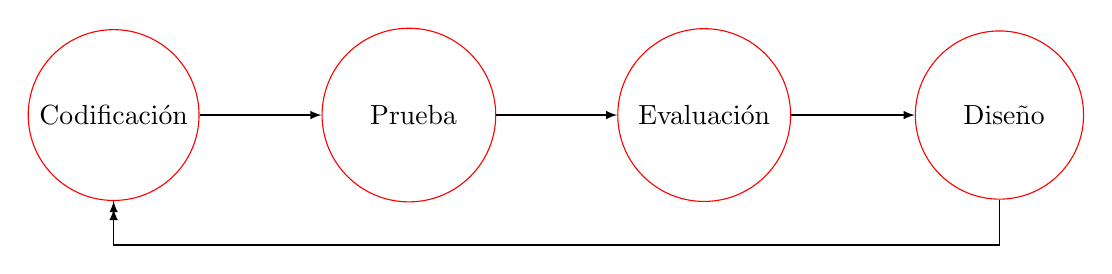
\begin{tikzpicture}[x=1.5cm, y=1.5cm]
	%\fill (-3.2,0) circle (0.1pt)node[anchor=east] {$20$};
	%\fill (3.2,0) circle (0.1pt)node[anchor=west] {$-20$};
    \node[circle,draw=red] (v1) at (-3.75,0) {Codificación};
    \node[circle,draw=red] (v2) at (-1.25,0) {\ \ \ \ Prueba\ \ \ \ };
    \node[circle,draw=red] (v3) at (1.25,0) {\ Evaluación\ \ };
    \node[circle,draw=red] (v4) at (3.75,0) {\ \ \ \ Diseño\ \ \ \ };
    \draw[color=black, -latex]  (v1) edge (v2);
    \draw[color=black, -latex]  (v2) edge (v3);
    \draw[color=black, -latex]  (v3) edge (v4);
    \draw (v4) -- (3.75,-1.1) -- (-3.75,-1.1) -> (v1);
    \draw[color=black, -latex]  (-3.75,-0.795) edge (v1);
\end{tikzpicture}
\end{center}
\caption{Iteración de etapas en XP.}
\label{fig:fig1}
\end{figure}

En la figura~\ref{fig:fig1} podemos observar un diagrama de las etapas estándar de XP. Si bien la primera etapa se corresponde normalmente con la codificación, en nuestro caso siempre lo ha sido el diseño. Así, para cada funcionalidad, se diseña la vista, se implementa la misma, a continuación se desarrolla y enlaza la lógica y por último se prueba. Se itera sobre estas etapas para cada vista y funcionalidad establecidas.
%
Se sigue así una planificación diseñada prácticamente para cada funcionalidad (planificación incremental), marcándose objetivos a muy corto plazo pero sin perder de vista el objetivo final: completar el sistema y su correcto funcionamiento.

Para concluir, hemos tratado de hacer nuestro código lo más adaptable posible, no sólo por el tipo de proceso de desarrollo elegido, sino también para facilitar futuras extensiones del sistema. Esto, sumado a todo lo contado en los anteriores párrafos, justifica que nuestro proceso de desarrollo se ajuste a XP y nos reafirma en considerar que esta  elección ha sido la más adecuada.

\section{MTQC: Mutation Testing for Quantum Computing}

MTQC son las siglas que dan nombre a nuestro sistema. Su principal funcionalidad es la de aplicar el proceso  de testing de mutaciones en distintos lenguajes cuánticos, en nuestro caso \qsh\ y \textit{Qiskit}.
%
La secuencia típica de acciones que seguirá  un usuario de MTQC consistiría en generar mutantes del programa deseado, verificar los mutantes creados, aplicar al programa original y a los mutantes seleccionados dadas una serie de test y cotejar los resultados para detectar test que revelan una discrepancia.

Sobre estas cuatro fases hemos establecido toda nuestra planificación, análisis y diseño del proyecto, tomando estas etapas como estructura de cara al desarrollo del sistema.

\subsection{Principales funcionalidades}

Aunque el desarrollo dirigido por casos de uso no es propio de XP, nos inspiramos en ellos para determinar las principales funcionalidades del sistema que podemos identificarlas con las fases recientemente nombradas. Podríamos definir alguna otra adicional, como la elección un lenguaje cuántico o el reinicio del programa, pero el grueso del contenido de MTQC lo recogen estas cuatro:

\begin{enumerate}
\item \textit{Generación de mutantes}. Se trata de la primera acción que el usuario debe realizar. Consta de dos entradas consistentes en dos listas: una del directorio de los archivos de código sobre los que se quiere realizar la mutación y otra de los operadores de mutación a aplicar. Arroja como salida una lista de mutantes vinculados al archivo original, el operador aplicado y la línea que sufrió la mutación. En caso de que la fabricación de un mutante provoque un error, se muestra por pantalla y se trata de generar el siguiente mutante.

\item \textit{Visualización de mutantes}. La precondición para que este caso de uso se pueda llevar a cabo es que previamente el usuario haya generado al menos un mutante. Toma como entrada una lista de mutantes con la que el usuario puede interactuar para así poder comparar el contenido de dicho mutante y el archivo original. El objetivo es que el usuario pueda tomar una decisión sobre si el mutante en cuestión es o no un candidato apto para ejecutar un test sobre él.

\item \textit{Testeo de mutantes}. Se trata del caso de uso principal del programa por importancia, cantidad y calidad del código asociado al mismo. Es necesario verificar la precondición de haber generado al menos un mutante para realizar cualquier acción sobre el mismo. Enumeraremos las entradas.
	\begin{itemize}
	\item Un archivo de código del lenguaje cuántico elegido en ese momento.
	\item Una función contenida en el archivo anterior.
	\item Una lista de todos los mutantes deseados para ejecución generados a partir de dicho archivo.
	\item Un tipo de testing a aplicar (determinista o probabilista).
	\item Un conjunto de test.
	\end{itemize}
	
La salida generará un conjunto de objetos que incluya los resultados obtenidos tras la ejecución de los test y sobre la muerte o no de los distintos mutantes que componen el conjunto pasado como parámetro.

\item \textit{Visualización de los resultados de los test}. Por último, tenemos la opción de que el usuario vea los resultados que los test han producido al ser aplicados a la función original y a los mutantes, determinar cuántos de ellos han sido matados y la eficacia de dichos test. La precondición indispensable para llevar a cabo esta visualización es haber llevado a cabo las acciones mencionadas en el anterior caso de uso. Toma como entrada un conjunto de objetos que gestionan los resultados de los test y muestra la información correspondiente, previo tratamiento, por pantalla. En el caso de que el test realizado haya sido de tipo probabilista, tomará también como entrada un porcentaje de confianza.
\end{enumerate}

Estas cuatro fases se han traducido en cuatro subsistemas bastante independientes. Aunque en un principio se pensó que las funcionalidades $3$ y $4$ conformarían un único subsistema, y estarían bajo una única vista, este planteamiento inicial cambió, principalmente, para no sobrecargar de información dicha vista y facilitar al usuario la lectura de los resultados, repartiendo las funcionalidades en diferentes subsistemas.

\subsection{Diseño}

Retomamos de nuevo las cuatro funcionalidades anteriores para componer la estructura principal del sistema. A la hora del diseño y desarrollo de MTQC se plantearon 4 subsistemas identificados cada uno de ellos con dichas funcionalidades.
%
Para implementarlos se optó por asignar a cada uno de ellos una pestaña visual independiente que quedan administradas bajo una misma vista conjunta. Esto se gestiona mediante el uso del patrón \textit{Modelo-Vista-Controlador} (MVC). Pese a no ser del todo necesario, por poseer una única vista, se ha implementado el patrón \textit{Observador} en el que la vista actúa como observador y la lógica como sujeto. Este patrón se ha usado para facilitar la adición de futuras interfaces, gráficas o no, que se pudieran desarrollar para  el sistema.

En algunas partes del código se ha  utilizado el patrón \textit{Factoría}. Por ejemplo, según el tipo de testing escogido, este crea una instancia de una subclase concreta que gestiona los resultados arrojados por el test. Por otra parte, somos conscientes de que este mismo patrón es útil en combinación con \textit{Observador} y MVC para facilitar, precisamente, implementar otras interfaces. Sin embargo, decidimos no aplicarlo como tal para facilitar el código. Pese a ello, de ser necesario, su ejecución no presentaría cambios significativos en el código, sino más bien algunas adiciones al mismo.

Detallaremos cada uno de estos subsistemas, pero antes vamos a exponer la jerarquía de paquetes que constituyen el sistema y unas breves indicaciones sobre su contenido y funcionalidad.

\subsubsection{Estructuración del código por paquetes}

\begin{itemize}
\item \texttt{model}. Contiene toda la lógica del programa. Además de todos los paquetes que aparecen a continuación, contiene las clases que conforman el patrón \textit{Observador} (\textit{Observer} y \textit{Observable}) y la clase \textit{Model} que gestiona el grueso de la lógica.
	\begin{itemize}
	\item \texttt{mutantoperator}. Recoge la clase abstracta \textit{MutantOperator} que gestiona un operador de mutación.
		\begin{itemize}
		\item \texttt{qiskit} Contiene todas las implementaciones de operadores de mutación creados para \textit{Qiskit}.
		\item \texttt{qsharp} Contiene todas las implementaciones de operadores de mutación creados para \qsh.
		\end{itemize}		 
	\item \texttt{mutant}. Contiene la clase \textit{Mutant} que gestiona un mutante tras su creación. Guarda ruta al archivo mutante, ruta al archivo original y línea de código que sufrió la mutación.
	\item \texttt{testing}. Contiene la clase abstracta \textit{Testing} que gestiona las características del tipo de testing a realizar, por ejemplo, si es o no determinista. También contiene sus implementaciones.
	\item \texttt{language}. Recoge clases que gestionan mutation testing y los lenguajes. Crea archivos ejecutables a partir de un mutante y una entrada de datos y los ejecuta.
	\item \texttt{files}. Contiene la clase \textit{TestFile} que gestiona los archivos finales creados por las clases del paquete \texttt{language}.
	\item \texttt{testresult}. Contiene la clase abstracta \textit{TestResult} que gestiona los resultados de la ejecución de los test y también sus implementaciones, una por cada implementación de \textit{Testing}.
	\end{itemize}
\item \texttt{view}. Está encargado de toda la vista del sistema.
	\begin{itemize}
	\item \texttt{mutantgeneartorview}. Contiene la vista correspondiente al primer subsistema.
	\item \texttt{mutantsviewer}. Contiene la vista correspondiente al segundo subsistema.
	\item \texttt{testcaserunnerview}. Contiene la vista correspondiente al tercer subsistema.
	\item \texttt{testresultview}. Contiene la vista correspondiente al cuarto subsistema.
	\item \texttt{tools}. Contiene algunas clases auxiliares utilizadas en la vista.
	\end{itemize}
\item \texttt{control}. Contiene la clase \textit{Control} que actúa como controlador del patrón \textit{MVC}.
\item \texttt{exception}. Recoge algunas excepciones del programa.
\item \texttt{main}. Recoge la clase \textit{Main} que contiene el método que inicia la ejecución del programa.
\end{itemize}

Estamos en disposición de hablar de cada subsistema con detenimiento y a esta tarea dedicaremos el resto de este capítulo. Mencionaremos los paquetes involucrados en cada uno de ellos, detalles de implementación, así como la aparición de problemas relevantes y la solución adoptada para ellos.

\subsubsection{Subsistema I: Generador de mutantes}

La generación de mutantes es el primer paso para realizar mutation testing. En la figura~\ref{fig:vista1} se presenta el aspecto de la vista asociada. La interfaz en su conjunto y cada una de las pestañas tiene un diseño simple, tratando de minimizar la cantidad de información presentada, para facilitar el uso y entendimiento por parte del cliente.

Los componentes de esta vista se encuentran en el paquete \texttt{view.mutantgeneratorview}, aunque además hace uso de clases del paquete \texttt{view.tools}. En concreto, \textit{JTableCheck}, que gestiona una tabla de  objetos de una determinada instancia junto a casillas verificadoras asociadas a booleanos y \textit{LogArea} que imprime información para el usuario. En cuanto a la lógica, los operadores se encuentran definidos en el paquete \texttt{model.mutantoperator}, y los mutantes generados se gestionan para su uso en el resto del programa mediante la clase \textit{Mutant} del paquete \texttt{model.mutant}.
\begin{figure}[t]
\begin{center}
\includegraphics[scale=0.45]{images/vista1}
\end{center}
\caption{Vista del subsistema generador de mutantes.}
\label{fig:vista1}
\end{figure}
La vista ofrece al usuario una lista de archivos en un determinado directorio que puede modificarse por el usuario. También aparece una lista de operadores de mutación acorde con el lenguaje cuántico seleccionado en ese momento. Tras la selección de los archivos y operadores se procede a llamar al controlador para que ordene a la lógica la creación de los mutantes. Para la generación de mutantes se ha implementado la técnica del {\it programador hábil}: sólo se aplica una mutación a cada archivo generado para simular que el programador ha cometido un único error. El proceso que sigue la lógica es sencillo: un operador contiene una secuencia de caracteres a ser buscada y otra con la que es reemplazada. Así, por cada archivo y operador, se generan tantos mutantes como veces se encontró dicha cadena. Todas estas acciones se realizan desde la clase \textit{Model}.

El mayor reto en esta fase del desarrollo consistía en el hecho de establecer cuando hemos encontrado una cadena de caracteres coincidente con la mutación que queremos incurrir. En el caso de \textit{Qiskit} esto es sencillo porque todas las instrucciones cuánticas son métodos que son llamados mediante un objeto perteneciente a la clase \textit{QuantumCircuit}. Así, todas las instrucciones siguen el formato
\begin{center}
\texttt{objeto.instrucción(...)}
\end{center}
y por tanto podemos buscar la cadena \texttt{.instrucción(} y sustituirla por \texttt{.mutación(} donde las palabras instrucción y mutación representan la conversión requerida. En el caso de \qsh\ no es tan sencillo, ya que las instrucciones tienen el formato
\begin{center}
\texttt{instrucción(...)}
\end{center}
así que no basta con sustituir \texttt{instrucción(} por \texttt{mutación(}. Supongamos que queremos realizar mutantes cambiando el operador de la puerta de \textit{Hadamard}, representado por la instrucción \texttt{H($\ldots$)}, por la puerta $X$. Si durante el proceso de reemplazo encontrásemos un método (por raro que fuera) acabado en H, por ejemplo \texttt{applyH($\ldots$)}, estaríamos generando un mutante en el que esa instrucción sería cambiada por \texttt{applyX($\ldots$)} que no es el efecto que deseamos. La solución es comprobar el carácter anterior y verificar que se trata de un salto de línea, un espacio o una tabulación.

Otro problema similar aparece con  los operadores de mutación aplicados a constantes de \qsh\ como \texttt{One} y \texttt{Zero}. La solución es, de nuevo, la comentada en el párrafo anterior pero aplicando dicha comprobación también al carácter posterior.

\subsubsection{Subsistema II: Visualizador de mutantes}

El segundo subsistema es el más simple de los cuatro. Se trata de una vista sencilla (figura \ref{fig:vista2}) que muestra la lista de mutantes generados y dos áreas de texto, que actúan como \textit{display} de los ficheros original y mutante. Si no se han generado mutantes previamente, la lista aparecerá vacía.

\begin{figure}[t]
\begin{center}
\includegraphics[scale=0.45]{images/vista2}
\end{center}
\caption{Vista del subsistema visualizador de mutantes.}
\label{fig:vista2}
\end{figure}

La lista de mutantes se gestiona mediante la clase \textit{JMutantList} en el paquete \texttt{view.tools}. El resto de componentes se gestionan desde las clases \textit{FileArea} y \textit{MutantsViewer} del paquete \texttt{view.mutantsviewer}. Además, la lista antes mencionada contiene no sólo el identificador del mutante, sino que también incluye la instancia al completo.

El funcionamiento de este subsistema es sencillo. El usuario debe pinchar sobre el mutante que quiera observar y la vista mostrará el contenido de las rutas a los archivos original y mutado sin necesidad de hacer llamada al controlador y, por tanto, tampoco al modelo. Tal vez en este caso no se estén siguiendo las directrices del patrón \textit{MVC} estrictamente, pero por su simplicidad optamos por este camino.

\subsubsection{Subsistema III: mutation testing y creación de test}

Es sin duda el componente más complejo del sistema. En él interviene gran parte de la lógica realizada para el proyecto. La funcionalidad se resume en ejecutar una elección de mutantes con unos test determinados para decretar qué porcentaje de ellos ha sido matado y la eficacia de los test utilizados.

\begin{figure}[t]
\begin{center}
\includegraphics[scale=0.45]{images/vista3}
\end{center}
\caption{Vista del subsistema mutation testing y creación de test.}
\label{fig:vista3}
\end{figure}

En la figura~\ref{fig:vista3} tenemos la vista que constituye el subsistema cuyos componentes se engloban dentro del paquete \texttt{view.testcaserunnerview} y que hace uso de las clases del paquete \texttt{view.tool}, \textit{TabbedTextArea}, que gestiona las entradas para los test que el usuario puede introducir mediante un sistema de pestañas; \textit{JTableCheck}, tabla que gestiona la selección de mutantes; \textit{TextField}, un simple campo de texto y \textit{LogArea}, que imprime información de la ejecución del programa al usuario.

Aunque el usuario podía en el primer subsistema seleccionar más de un archivo para aplicar mutaciones sobre él, para realizar mutation testing debemos hacerlo, en este caso, de manera individual. Además, los archivos que MTQC genera para ejecutar todos los test se almacenan en una carpeta auxiliar. Por tanto, el programa que sirve de base para el proceso de testing de mutaciones no podrá usar archivos o librerías que no estén en el directorio por defecto del lenguaje correspondiente. Para solucionar esto, el usuario puede incluir la ruta a los archivos necesarios en el propio programa. Por ejemplo, en \textit{Python} puede hacerse con el siguiente código:

%\begin{figure}[t]
\begin{lstlisting}[language=Python]
import sys
sys.path.insert(0, "path_to_your_package")
\end{lstlisting}
%\caption{Código para añadir una nueva ruta donde \textit{Python} buscará módulos.}
%\label{fig:code1}
%\end{figure}

Cabe destacar que, en general, los programas cuánticos rara vez alcanzan una extensión suficiente para ser modulados en varios archivos y esta {\it complicación} no debería ser un problema en la inmensa mayoría de los programas con los que se trabaje.

Así, la primera decisión que ha de tomar el usuario es la de elegir el archivo deseado. En la vista se muestran los correspondientes a la ruta seleccionada en el primer subsistema. Tras la elección, se llama al controlador para que la lógica realice dos tareas. La primera es obtener todos los mutantes generados a partir del archivo seleccionado; la segunda es devolver todas las funciones encontradas en el archivo.

El usuario debe ahora realizar el resto de la configuración: elegir los mutantes a ejecutar, la función de llamada, el tiempo límite para la ejecución de cada test (para evitar ejecuciones infinitas debido a que nos hayamos quedado en un bucle a causa de la mutación), el tipo de testing, el número de ejecuciones, si este último es probabilista y, por último, las entradas o test.

En cuanto al tipo de testing, nuestra herramienta incluye dos opciones por defecto: uno determinista, que hemos denominado {\textit{QStateTesting}}, y otro probabilista, {\textit{ProbabilisticTesting}}. El primero compara las probabilidades arrojadas por los estados finales del sistema cuántico. Supongamos que una función sobre un sistema cuántico de un qubit devuelve $\frac{1}{\sqrt{2}}\ket{0}+\frac{1}{\sqrt{2}}\ket{1}$ mientras que el mutante devuelve $\frac{1}{\sqrt{2}}\ket{0}-\frac{1}{\sqrt{2}}\ket{1}$, este test evalúa las probabilidades de cada estado, que en ambos casos son de $\frac{1}{2}$ para $\ket0$ y un $\frac{1}{2}$ para $\ket1$. Por tanto, no se mataría al mutante pese a que los estados cuánticos no son idénticos.
%
Huelga decir que este primer tipo de testing solo es posible si se ejecuta sobre un simulador en un computador clásico. Para su implementación, en el caso de \qsh\ hemos hecho uso de la instrucción \texttt{DumpMachine()} que imprime en un fichero o pantalla el estado cuántico en ese momento, mientras que el simulador \textit{StatevectorSimulator} de \textit{Qiskit} permite de igual modo acceder a dicha información.

El segundo tipo de testing, \textit{ProbabilisticTesting}, compara la salida final de la función que, generalmente, será la medición de uno o más qubits. Por tanto, esta salida puede ser probabilista y su ejecución debe ser realizada en repetidas ocasiones con el fin de conseguir una certeza estadística sobre la muerte o no del mutante. Dicho testing puede ser aplicado en computadoras cuánticas usando \textit{Qiskit}, basta con seleccionar una máquina de \textit{IBM} disponible para la ejecución escribiendo el código correspondiente en la entrada. Sin embargo, hay que tener en cuenta que la disponibilidad de estas computadoras es muy limitada y las ejecuciones mensuales también lo son, así que se podría demorar bastante la obtención del resultado.

Como vimos en el capítulo anterior, la inicialización del estado cuántico deseado supone un problema añadido respecto de la computación clásica. El usuario debe dar una secuencia de puertas para conseguir el estado de entrada deseado. En el caso de \textit{Qiskit}, existe una función del circuito cuántico (\textit{QuantumCircuit}), \texttt{initialize()}, que permite inicializar el circuito en el estado deseado, siempre que el simulador utilizado sea \textit{StatevectorSimulator}.

\begin{figure}[t]
\begin{lstlisting}[language=Python]
from qiskit import *
import numpy as np

qr = QuantumRegister(3)
qc = QuantumCircuit(qr)
init = [complex(0, 1/np.sqrt(2)), 0, 0, complex(1/np.sqrt(2), 0), 0, 0, 0, 0]
qc.initialize(init, qr)
\end{lstlisting}
\caption{Inicialización de un circuito cuántico mediante un vector complejo en \textit{Qiskit}.}
\label{fig:code2}
\end{figure}

El código de la figura~\ref{fig:code2} inicializa el circuito cuántico de $3$ qubits en el estado $\frac{i}{\sqrt{2}}\ket{000}+\frac{1}{\sqrt{2}}\ket{011}$. Nótese que el vector dado como ejemplo tiene norma uno; en otro caso la ejecución arrojaría un error.

En cualquier caso, la preparación de la entrada requiere un tratamiento previo. Para tratar esta entrada hemos facilitado dos métodos. El primero es mediante la carga de un archivo de texto en el que cada caso es separado por una línea con la secuencia de caracteres \textbf{***} y cada caso tiene que tener la estructura del segundo método que mencionamos a continuación. El segundo es un sistema de pestaña. Por defecto aparece una pestaña con un ejemplo estructural a seguir y en el caso de de añadir una nueva, aparece con una copia del contenido de la seleccionada previamente. El código dado por defecto para \textit{Qiskit} está reflejado en la figura \ref{fig:code3}.

\begin{figure}[bt]
\begin{lstlisting}[language=Python]
def init ():
	cr = ClassicalRegister(1)
	qr = QuantumRegister(1)
	qc = QuantumCircuit(qr, cr)

	# Initialize with desired quantum gates or QuantumCircuit.initialize() method

	# Call your method

	ex = execute(qc, backend = Aer.get_backend('statevector_simulator'))

	# Add any operations if needed
	
	return next(iter(ex.result().get_counts())) # Change desired return
	#return pow(abs(ex.result().get_statevector()), 2) # If probabilistic test chosen
\end{lstlisting}
\caption{Código dado por defecto en MTQC para inicializar un test en \textit{Qiskit}.}
\label{fig:code3}
\end{figure}

Según lo deseado, podemos modificar el número de registro clásicos (\textit{ClassicalRegister}) y cuánticos (\textit{QuantumRegister}), añadir la inicialización deseada en cada caso y debemos llamar al método elegido. Por último, habrá que comentar uno de los dos \texttt{return} en función del tipo de testing elegido, según se indica, o incluso puede ser cambiado para devolver otro tipo de datos si se desea. Es importante recalcar que \textit{Qiskit} construye un circuito con el uso de métodos de aplicación de puertas, pero realmente ese circuito no se ejecuta hasta que no se llama a la instrucción \texttt{execute($\ldots$)}. Si se llama a esta función  en el método que se está utilizando como base del proceso de testing, basta con comentar o borrar la línea de código correspondiente de la figura~\ref{fig:code3}.
%
En cualquier caso, debemos mantener la tabulación establecida y no cambiar el nombre del método definido en la primera línea, pues se llama para poder  inicializar la entrada. Si se opta por la introducción vía archivo, este método tiene que estar definido para cada caso de igual modo.

\begin{figure}[tb]
\begin{lstlisting}[language=c++]
operation MainQuantum() : // Define main function output type {

	// Select desired Qubit number to be used
	using (register = Qubit[2]) {

    	// Inicialize variables and Qubits

    	// Call method and save output

    	// If probabilistic test chosen.
    	// DumpMachine("temp.txt");

    	// Reset all qubits to Zero state
    	ResetAll(register);

    	// Return output
	}
}
// Define any other operation if needed as input
\end{lstlisting}
\caption{Código dado por defecto en MTQC para inicializar un test en \qsh.}
\label{fig:code4}
\end{figure}

Para el caso del lenguaje \qsh\ tenemos indicaciones similares (véase figura \ref{fig:code4}). De nuevo, debemos mantener la estructura general y modificar lo necesario siguiendo las indicaciones, ya haya sido elegido el método de entrada mediante el uso de la vista de pestañas o mediante la carga de archivo.

Tenemos así todo listo para proceder: archivo, método, mutantes, tipo de testing y conjunto de test que vamos a aplicar, entre otros. Todos estos datos se gestionan con las clases mencionadas anteriormente para cada uno de ellos. El usuario está listo para ejecutar los test y la vista llama al controlador que preprocesa los datos antes de enviárselos a la lógica. El primer objetivo es preparar nuevos archivos que añadan las entradas establecidas a los archivos a ejecutar: mutantes y original. Dichos archivos son creados por las clases del paquete \texttt{model.language} y gestionadas por la clase \textit{TestFile} del paquete \texttt{model.files}.

El siguiente paso consiste en generar un archivo principal en \textit{Python} que se ejecutará mediante una llamada al sistema (por tanto, el usuario debe tener agregado \textit{Python} en su \textit{path}) y que llamará a todos los archivos generados en el paso anterior para obtener las salidas producidas por los test.
%
Tras ser estos ejecutados, MTQC recoge las salidas resultantes de la ejecución asignándolas al archivo original o mutante y a uno de los test según corresponda. Esta gestión de datos se realiza mediante una de las clases del paquete \texttt{model.testresult}, según el tipo de testing elegido.

Para acabar, todos los archivos generados durante esta fase son borrados y se manda una actualización de los resultados obtenidos al último subsistema que veremos a continuación.

\subsubsection{Subsistema IV: Visualizador de resultados}

En último lugar tenemos el subsistema dedicado a visualizar los resultados. La vista  está consituida por un sencillo sistema de pestañas, una para cada test, que contiene una tabla donde se comparan los resultados y se indica qué mutantes han muerto y cuáles no (véase figura \ref{fig:vista4}).
%
Los componentes de la vista se encuentran íntegramente en el paquete \texttt{view.testresultview} a excepción de la clase \textit{ResultTable}, que gestiona cada tabla, del paquete \texttt{view.tools}. Como hemos mencionado, los resultados que se muestran en esta vista se actualizan automáticamente al final de la ejecución del subsistema anterior.

\begin{figure}[tb]
\begin{center}
\includegraphics[scale=0.45]{images/vista4}
\end{center}
\caption{Vista del subsistema visualizador de resultados.}
\label{fig:vista4}
\end{figure}

Además, el usuario puede modificar la confianza utilizada para matar a un mutante en un test probabilístico. Supongamos que tenemos un total de $n$ estados posibles ($\ket0,...,\ket{n-1}$) en cierto sistema cuántico y hemos ejecutado $k$ veces tanto el archivo original como el mutante. Definimos las probabilidades de medición del estado cuántico $\ket i$ para el archivo original como
$$p_{\ket i,o}=\dfrac{f_{\ket i,o}}{k}
$$
donde $f_{\ket i,o}$ denota el número de veces que la salida del programa original fue el estado $\ket i$. Análogamente, para cierto  mutante $m$ definimos las probabilidades de medición del estado cuántico $\ket i$ como
$$
p_{\ket i,m}=\dfrac{f_{\ket i,m}}{k}
$$
donde $f_{\ket i,m}$ denota el número de veces que la salida del mutante $m$ fue el estado $\ket i$. Así un mutante $m$ muere si se verifica
$$
\max \{|p_{\ket i,o}-p_{\ket i,m}|:0\leq i\leq n - 1\}> c
$$
donde $c$ denota el parámetro de confianza, que puede ser modificado por el usuario de nuestro sistema. Obviamente el máximo del conjunto anterior está comprendido entre $0$ y $1$, por estarlo las probabilidades definidas anteriormente. El parámetro de confianza en MTQC por defecto es del $1\%$, pero puede modificarse para aplicar otro porcentaje que el usuario considere más adecuado. Tras esto, se contactará con la clase \textit{Model} de la lógica que solicitará a cada instancia de la clase \textit{TestResult} que recalcule la muerte o no del mutante en función del nuevo valor indicado y comunicará a la vista los resultados.